\chapter{Lecture 6}
Suppose we have $f:\{\pm1\}^n\to \{\pm 1\}$.
\begin{definition}[Sensitivity]
    $\forall\ i\in[n]$ and $x\in \{\pm \}^n$ we say $i$ is a sensitive / pivotal coordinate at $x$ for $f$ if $$f(x)\neq f(x^{\oplus i})$$where $x^{\oplus i}\coloneqq (x_1,\dots, x_{i-1}, -x_i,x_{i+1},\dots, x_n)$
\end{definition}
\begin{definition}[Influence]
    $\ifl_i[f]=\underset{x\in \{\pm 1\}^n}{Pr}[f(x)\neq f(x^{\oplus i})]$
\end{definition}


\begin{center}
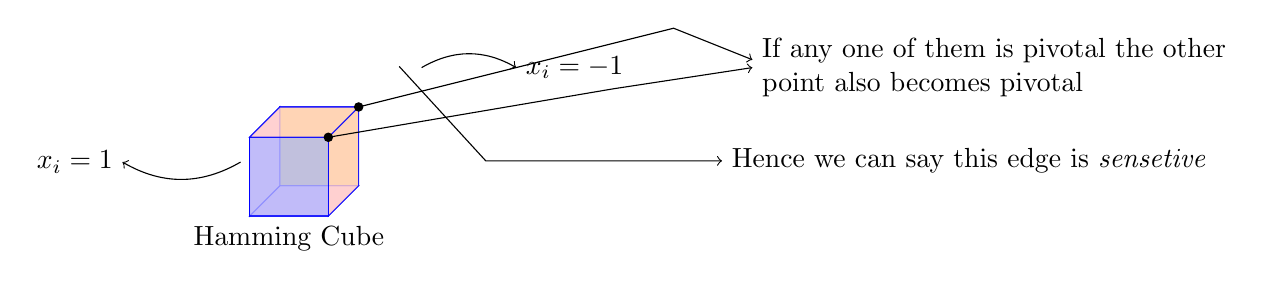
\begin{tikzpicture}
\coordinate (O) at (0,0,0);
\coordinate (A) at (0,\Width,0);
\coordinate (B) at (0,\Width,\Height);
\coordinate (C) at (0,0,\Height);
\coordinate (D) at (\Depth,0,0);
\coordinate (E) at (\Depth,\Width,0);
\coordinate (F) at (\Depth,\Width,\Height);
\coordinate (G) at (\Depth,0,\Height);

\draw[blue,fill=red!20,opacity=0.6] (O) -- (C) -- (G)  node[midway,  below, color= black, opacity=1]{Hamming Cube} -- (D) -- cycle;% Bottom Face
\draw[blue,fill=yellow!80,opacity=0.8] (O) -- (A) -- (E) -- (D) -- cycle;% Back Face
\draw[blue,fill=red!10] (O) -- (A) -- (B) -- (C) -- cycle;% Left Face
\draw[blue,fill=red!20,opacity=0.8] (D) -- (E) -- (F) -- (G) -- cycle;% Right Face
\draw[blue,fill=blue!30, opacity=0.8] (C)  -- (B)  -- (F)  -- (G)   -- cycle;% Front Face
\draw[blue,fill=red!20,opacity=0.8] (A) -- (B) -- (F)  -- (E) -- cycle;% Top Face
\draw[->, bend left] (1.8,1.5,0) to[bend left=30] (3,1.5,0) node[right] {$x_i=-1$}; 
\draw[->, bend left] (-0.5,0.3,0) to[bend left=30] (-2,0.3,0) node[left] {$x_i=1$}; 
\filldraw (E) circle (1.5pt);
\filldraw (F) circle (1.5pt);
\draw[->] (E) -- (5,2,0) -- (6,1.6,0);
\draw[->] (F) -- (5,2,2) -- (6,1.5,0) node [right, text width=6cm]{If any one of them is pivotal the other point also becomes pivotal};
\draw[->] (1.9,1.9,1) -- (3,0.7,1) -- (6,0.7,1) node[right]{Hence we can say this edge is \textit{sensetive}};
    \end{tikzpicture}
\end{center}

So $\ifl_i[f]=\frac{\#\text{sensitive edge wrt $i$}}{\#\text{edges in direction of $i$}}$.
\begin{lemma}\label{effective-fourier-coeff}
	$\eff_i[f]=\hat{f}(\{i\})$
\end{lemma}
\setlength{\parindent}{0cm}

\textbf{Notation:} For $x\in \{\pm 1\}^n$ denote $$x^{i\to 1}\coloneqq (x_1,\dots, x_{i-1},1,x_{i+1},\dots, x_n)\qquad \text{and}\qquad x^{i\to -1}=(x_1,\dots, x_{i-1}, -1,x_{i+1},\dots, x_n)$$
\begin{definition}[Partital Derivative in direction of $i$]
	For $f:\{\pm 1\}^n\to \{\pm 1\}$ then the partial derivative of $f$ in direction of $i$ is $$D_i(f)(x)=\frac{f(x^{i\to 1})-f(x^{i\to -1})}{2}$$
\end{definition}

\textbf{Observation:} $D_if(x)=\begin{cases}
	\pm 1 & \text{$i$ is sensitive}\\
	0 & \text{otherwise}
\end{cases}$

\begin{lemma}
	\begin{enumerate}
		\item $\ifl_i[f]=\E_{x}\left[(D_if)^2\right]$
		\item $\eff_i[f]=\E[D_if]$
	\end{enumerate}
\end{lemma}
\begin{definition}[Total Influence and Effect]For a function $f:\{\pm 1\}^n\to \{\pm 1\}$
	\begin{itemize}
		\item $\ifl[f]\coloneqq \sum\limits_{i=1}^n \ifl_i[f]$
		\item $\eff[f]\coloneqq \sum\limits_{i=1}^n \eff_i[f]$
	\end{itemize}
\end{definition}
\begin{note}[Fourier Expansion of Derivative]For a function $f:\{\pm 1\}^n\to \{\pm 1\}$	$$D_if=\sum\limits_{i\notin S\subseteq [n]}\hat{f}(S\cup \{i\})\chi_S$$
\end{note}Hence we have $\widehat{D_if}(S)=\begin{cases}
\hat{f}(S\cup \{i\})&\text{when $i\notin S$}\\
0 & \text{otherwise}
\end{cases}$
\begin{corollary}[Parseval for $D_if$]\label{influence-fourier-coeff}
	$\ifl_i[f]=\sum\limits_{i\in S\subseteq [n]} (\hat{f}(S))^2$
\end{corollary}
\begin{question}[ $\ifl_i{[Parity_n]}$]
	Consider the function $Parity_n:\{\pm 1\}^n\to \{\pm 1\}$ where $Parity_n=x_1\cdots x_n$ then  calculate $\ifl_i[Parity_n]=1$
\end{question}

\textbf{Observation:} Maximum influence is achieved by $Parity_n$

\begin{question}[ $\ifl_i{[Maj_n]}$]
	Consider the function $Maj_n:\{\pm 1\}^n\to \{\pm 1\}$ where $Maj_n=x_1\cdots x_n$ then  calculate $\ifl_i[Maj_n]=\frac{c}{\sqrt{n}}$ for some constant $c$
\end{question}

\begin{question}[ $\ifl_i{[Tribes_{s,w}]}$]
	Consider the function $Tribes_{s,w}=\underset{i=[s]}{\bigvee}(\bigwedge\limits_{j\in w}x_{i,j})$ where $s,w\in \mathbb{N}$  calculate $\ifl_i[Tribes_{s,w}]=\frac1{2^{w-1}}\left( 1-\frac1{2^w} \right)^{s-1}$
\end{question}

\begin{note}[Kahn-Kalai-Linial 89]Let $f:\{\pm 1\}^n\to \{\pm 1\}$ with $\Var[f]=\Omega(1)$ then $\exists\ i\in[n]$ such that $\ifl_i[f]=\Omega\left( \frac{\log n}{n} \right)$
\end{note}
Here $$\langle f,f\rangle=1=\sum\limits_{S\subseteq [n]}(\hat{f}(S))^2\quad\text{and}\quad \Var[f]=\sum\limits_{S\neq \emptyset,S\subseteq [n]}(\hat{f}(S))^2$$

\begin{definition}[Sensitivity of a Point]
	Let $f:\{\pm 1\}^n\to \{\pm 1\}$ and $x\in\{\pm 1\}^n$. We define $\sen_f(x)$ to be the number of sensitive edges incident to $x$.
\end{definition}

\begin{lemma}
	$\ifl[f]=\E_{x}[\sen_f(x)]$
\end{lemma}
\begin{proof}
	\begin{align*}
		\E_x[\sen_f(x)] & = \frac1{2^n}\sum\limits_x\sen_f(x)\\
		& = \frac1{2^n}\sum\limits_{x}\sum\limits_{\substack{i\in [n]\\ f(x)\neq f(x^{\oplus i})}}1\\
		&= \sum\limits_{i\in[n]}\frac1{2^n}\sum_{\substack{x\\ f(x)\neq f(x^{\oplus i})}}1\\
		& = \sum_{i\in[n]}\ifl_i[f]=\ifl[f]
	\end{align*}

Another way of seeing this is since each sensitive edge is incident to two points in the boolean cube, $\sum\limits_x \sen_f(x)$ is the twice the $\#$sensitive edges $=2^n\ifl[f]$
\end{proof}
\begin{lemma}
	$\ifl[f]=\sum\limits_{S\subseteq [n]}|S|(\hat{f}(S))^2$
\end{lemma}
\begin{proof}
	From \hyperref[influence-fourier-coeff]{Corollary \ref{influence-fourier-coeff}} in $\ifl[f]$ the term $(\hat{f}(S))^2 $ appears for all $i\in S$. 
\end{proof}
\begin{theorem}
	Let $n$ is odd. $Maj_n$ is an unique function which maximizes effectiveness.
\end{theorem}
\begin{proof}
	We have $\eff[f]=\sum\limits_{i=1}^n \eff_i[f]$. Now we also have from  \hyperref[effective-fourier-coeff]{Lemma \ref{effective-fourier-coeff}} that $$\eff_i[f]=\hat{f}(\{i\})=\langle f,\chi_i\rangle=\langle f,x_i\rangle$$Therefore we have $$\eff[f]=\left\langle f,\sum_{i\in[n]} x_i\right\rangle$$
	\setlength{\parindent}{1cm}
	
	Therefore the function whose norm is 1 and maximizes $\left\langle f,\sum\limits_{i\in [n]}\right\rangle$ is of same sign with $\sum x_i$. Only $f$ that maximizes will be $sign \left(  \sum\limits_{i=1}^n x_i  \right)$ and notice $sign \left( \sum\limits_{i=1}^n x_i\right)=Maj_n$.
\end{proof}